% !TeX spellcheck = en_UK


%
%\pg
%There exists a wide variety of methods used in imaging, from the venerable CLEAN algorithm\footnote{For an excellent beginner's introduction to CLEAN, the author heartily recommends \url{https://www.cv.nrao.edu/~abridle/deconvol/node7.html}} to cutting-edge compressed sensing and subspace deconvolution methods. We will begin this section by introducing a mathematical framework in which the problem of deconvolution can be understood, and proceed, from there, to discuss some of the deconvolution algorithms which can be used.
%
%\pg
%The formalism used in this section is based, in part or in whole, on that used by Cyril Tasse in [DDF paper].

\section{A Brief Introduction to Radio Astronomy}
\pg
Radio astronomy consists of observing the electromagnetic emission of astrophysical\footnote{And, famously, attempting to observe ``intelligent" sources \citepads[cf]{2017AAS...22911604E}} sources at very long wavelengths by means of radio antennas. These antennas measure a voltage proportional to variations in the electromagnetic field in all the directions they are sensitive to. Since astrophysical signals are weak, a good sensitivity is necessary. Achieving good sensitivity with radio antennas means having a very large collecting area - in this respect, they behave exactly the same way as optical telescopes. Similarly, when well-designed, they are diffraction-limited - this means that, once again like optical telescopes, their resolution is limited by their diameter.

\pg
However, because radio frequencies are so much lower, achieving a resolution comparable to e.g. the HST requires extremely large dishes. While there exist telescopes, both old and new, which work on this principle (from Arecibo Observatory, shown in \cref{fig.arecibo}, to the upcoming FAST telescope in China, shown in \cref{fig.FAST}), the associated technical difficulties (pointing is complex business, as are the associated optics requirements; maintenance costs are high, etc...) have made the single-dish approach prohibitive.

\begin{figure}[ht]
\centering
\begin{subfigure}{.48\textwidth}
\resizebox{\hsize}{!}{\includegraphics{images/20151101114231-0_8e7cc_c7a44aca_orig.jpg}}
\caption{\label{fig.arecibo} Arecibo telescope, in Puerto Rico.}
\end{subfigure}
\hfill
\begin{subfigure}{.48\textwidth}
\resizebox{\hsize}{!}{\includegraphics{images/FastTelescope_8sep2015.jpg}}
\caption{\label{fig.FAST} FAST telescope, in China}
\end{subfigure}
\caption{\label{fig.singleDishes} Examples of large single-dish radio telescopes.}
\end{figure}

\pg
One way to move past this technical limitation is to resort to interferometry: this is the topic of this section.

\section{An Observer's Perspective of Radio Interferometry}

\pg
Astronomers who request observation time on interferometric arrays are generally not experts in the theory and operation of these arrays. This is a simple consequence of scientific division of labour. This thesis is written from the perspective of an ``expert" user: one who specialises in understanding interferometric arrays and reducing their data, rather than their subsequent analysis. However, it can be very helpful to contextualise this perspective in the experience of other scientists, which is what this section aims to do. This is simply to highlight the conceptual structure of a radio interferometric observation, and where the concepts outlined in this chapter fall in the overall pattern. In other words, it is best understood as a guide to see where a given section's topic slots into the overall production of an image made from visibilities.
\pg
LOFAR data can be acquired through observation or via the Long-Term Archive. The worst of this data will already be flagged. Users can thus generally proceed directly to calibration. Because there is no guarantee of sufficient signal-to-noise in the ``target field" (the object that the astronomer is actually interested in), it is standard practice to observe a calibrator source for 5 minutes before and after each observation. Such sources typically need to be bright and unresolved for the interferometer being used. Because they are bright and at phase centre for the 5-minute observation, the SNR when solving for calibration solutions for these 5 minutes will tend to be quite good. These solutions will then be interpolated between the 5 minutes onto the 8-hour observation. Calibration will be described in \cref{section.calibration}.

\pg
So far, the astronomer will have worked entirely with visibilities. However, generally speaking, the aim will be to get information on the object's brightness distribution at the observing frequency. This will require \emph{imaging}: going from visibilities to the image-plane. This can be done through a variety of tools, but will generally involve deconvolution. Imaging will be the subject of the rest of this chapter, and deconvolution will be described in more detail in \cref{section.clean}.

\pg
After obtaining the initial image, it may be desirable to perform a few rounds of self-calibration \citepads[cf.]{2018arXiv180505266B} on the target field. This consists of extracting a model from the initial image and using it as a new calibration model, then re-imaging. Doing this will usually dramatically improve the final image. 

\pg
The framework for interferometric calibration is complex, and understanding it requires a good grasp on interferometry itself. For now, we will assume that calibration has been performed perfectly, and that the gain-corrections have been applied to the voltage measured by our antennas. We therefore work with the true signal from astrophysical sources until \cref{section.RIME}.



\section{Interferometry: Bypassing the Diffraction Limit}

\pg
There are two quantities of interest to all astronomers: sensitivity and angular resolution\footnote{Other kinds of resolutions - in time and frequency, for example - are also extremely important to many astronomers, but are not what concern us here.}. An instrument's sensitivity is a function of its collecting area\footnote{It is also a function of technological factors, of course, but \emph{ceteris paribus}, a more sensitive telescope means a telescope with a wider collecting area}. Resolution, for well-designed instruments\footnote{By this, we mean that we assume that an instrument is also designed to optimise resolution.}, is limited by diffraction in the absence of atmospheric effects. This introduces specific issues in the radio domain. Radio waves have very long wavelengths - often comparable to meters, rather than the $\sim100-1000$nm wavelengths of optical light. Achieving a resolution comparable to those of optical telescopes would thus require making telescopes with apertures tens of millions of times larger than those already titanic instruments!

\pg
In practice, this technical constraint on resolution is one that astronomers are very interested in overcoming. This technical limitation therefore demands a technical solution. In practice, this solution consists of recourse to interferometric techniques. Indeed, interferometry can be thought of as the construction of a "sparse" dish, as illustrated in \cref{fig.aperture.synthesis}.

\begin{figure}[ht]
\centering
\begin{subfigure}{.43\textwidth}
\resizebox{\hsize}{!}{\includegraphics{images/baseline-resolution.png}}
\caption{\label{fig.baseline.image} A pair of dishes can surpass the resolution limit of its components.}
\end{subfigure}
\hfill
\begin{subfigure}{.43\textwidth}
\resizebox{\hsize}{!}{\includegraphics{images/sparseArray.png}}
\caption{\label{fig.arecibo.vla} With enough pairs of dishes, it is possible to synthesise a much larger dish.}
\end{subfigure}
\caption{\label{fig.aperture.synthesis} Illustration of the underlying principle of interferometry. The 27 dishes of the VLA can be thought of as "synthesising" a similar circular dish as Arecibo. This idea is the reason why radio interferometry is historically known as "aperture synthesis" in the literature of radio astronomy. \cref{fig.baseline.image} is copyrighted by Addison Wesley.} % \textcolor{red}{CHANGE FIG B. AS THE ELLIPSE IS NOT SEE-THROUGH}}
\end{figure}

\pg
Interferometric measurements are made as follows: the elements of the interferometric array (which can be single dishes or phased arrays\footnote{Described in \cref{sec.visibility}} of smaller antennas) measure a voltage. This voltage is correlated between antennas, as will be described shortly. Each of these correlations correspond to a single Fourier mode of the sky, as per the Zernike-van Cittert theorem (cf. \cref{sec.imag.psf}). They must be calibrated, by comparing the observations of a calibrator source and modelled visibilities. Calibration is described in much greater detail in \cref{section.RIME}. Then, the calibrated visibilities are used to reconstruct an image of the sky, which often requires deconvolution due to the sparsity of interferometric arrays.

\pg
The resolution improvement of interferometers does thus not come for free. To better understand the cost of interferometry, we will cover calibration after explaining the particularities of interferometers. We will begin with the properties of their core component: the baseline.

\subsection{The Baseline}

\pg
To define the baseline, we must begin by considering the geometric properties of an interferometric array. For now, let us assume that we are observing the sky above the array, a practice known as drift-scanning. A baseline then consists of the vector subtraction of the positions, in 3-dimensional space, of its two constituent antennas. Note that each antenna pair therefore has 2 corresponding baselines, since for each pair of antennas A and B we create baselines AB and BA. These distance vectors are then divided by the observing wavelength to give a dimensionless set of coordinates, known as $(u,v,w)$. These coordinates define the baseline entirely. 

\subsection{The Visibility}\label{sec.visibility}

\pg
We have defined what a baseline corresponds to: a vector coordinate in $(u,v,w)$-space. To each baseline we associate a measurement, which we call the \emph{visibility}. 
\begin{figure}[ht]
\centering
\includegraphics[width=.7\textwidth]{images/visibility-creation.png}
\caption{\label{fig.visibility} There are two ways to combine the voltages from two antennas into a visibility: they are sum-correlation and $\pi$-correlation. In this manuscript, we will only concern ourselves with the latter. Image credit: Julien Girard}
\end{figure}
The visibility associated with baseline $\mathbf{b}_{AB}$ is created by taking the voltage $V_A$ measured by antenna A, multiply it by the complex conjugate $V_B^*$ of the voltage measured by antenna B, average over the correlator dump time (i.e. the time over which the measurement is made). This scalar quantity is associated to the baseline position vector $\mathbf{b}_{AB}$. In other words:
\begin{align}
\mathbf{b}_{AB} &= \frac{\mathbf{x}_{B}-\mathbf{x}_{A}}{\lambda_\mathrm{obs}}\\
V_{AB}          &= \langle V_{A} V_{B}^*\rangle_{\delta t, \delta \nu} 
\end{align}
where $\langle \cdots \rangle_{i}$ denotes an averaging over quantity $i$. We see that a visibility is a complex vector quantity. We also see that $\mathbf{b}_{AB} = \mathbf{b}_{BA}^*$: the information of the visibility associated with baseline BA is contained in the visibility associated with baseline AB. This means that in practice, only half of the visibilities ever need be stored. What does the visibility measurement correspond to?
\begin{figure}[ht]
\centering
\includegraphics[width=.5\textwidth]{images/visibility-measure.png}
\caption{\label{fig.visibility.measure} Here, we assume that there are only two sources in the sky whose signal can be measured by our antennas. The final visibility is the sum of the visibilities associated with each individual source. Image credit: Julien Girard \textcolor{red}{add reference to julien's phd}}
\end{figure}

\pg
Different astrophysical sources are located very far apart, and so their signals do not interfere. They are measured additively in both antennas. Provided that the signal from both sources is coherent when observed by the dishes, the correlation between the voltages measured by antennas A and B will simply be the sum of the voltage correlations associated with individual sources. This is shown in \cref{fig.visibility}: the radio signal from two different sources, at two different locations, is picked up simultaneously by both radio antennas. Because only the correlation between both antennas is measured, the signals do not interfere: if the signal from each source gives a voltage $V_{p}^s$ for antenna $p$, then the additive property of electric fields means that the total visibility measured by baseline $pq$ can be written as:
\begin{align}
V_{pq}  &= \langle \left(\sum_{s} V_{p}^s\right) \left(\sum_{s} (V_{q}^s)\right)^*  \rangle_{\Delta t} \\
        &= \langle \sum_{s,s'} V_{p}^s (V_q^{s'})^*  \rangle_{\Delta t}\\
        &= \langle \sum_s V_{p}^s (V_q^{s})^* \rangle_{\Delta t} + \underbrace{\langle \sum_{s,s'\ne s} V_{p}^s (V_q^{s'})^* \rangle_{\Delta t}}_{=0} \label{eq.spatial.incor}
\end{align}
where the fact that signal from different sources is not coherent means that we average out cross-contributions (i.e. signal from $s\ne s'$). 
%\begin{align}
%V_{pq}&=\langle \left(\sum_{s} V_{p}^s\right) \left(\sum_{s} V_{q}^s \right)^* \rangle_{\Delta t} \right)\\
%      &=\langle\sum_{s,s'} \left( V_p^s\left(V_q^{s'}\right)^* \rangle_{\Delta t}
%\end{align}

\pg
Note that in Fig. \ref{fig.visibility.measure}, neither source is at the zenith. This introduces the notion of the \emph{effective baseline} which is shorter than the \emph{physical baseline} when measuring a signal from a source that is not at the zenith. Sources in different positions in the sky will be measured by an interferometric array, but the same array will have different effective baselines for different sources. To point an interferometric array in a specific direction in the sky, one must introduce a phase delay in each antenna (or, for fundamental interferometer elements such as the LOFAR tiles or NenuFAR, by playing with the cable length between each dish and the correlator). Because the phase needs to be properly sampled to limit information loss, a process known as fringe stopping\footnote{see \href{https://casper.berkeley.edu/astrobaki/index.php/Fringe_Stopping}{here} for more information. Fringe stopping consists of measuring the beat between a predicted fringe rate (i.e. the period of the visibility sine wave corresponding to a point source out of phase centre; if the position of an array's antennas is well-known, this can be modeled accurately) and the actual fringe rate (i.e. the fringe rate corresponding to the true period of the visibility sine wave). The difference between the two is a function of how well the antennas' positions are known. If they are well-known, then the phase information can still be measured, even without very fine sampling in time. } must be used to avoid taking a measurement every few milliseconds. The position of sources are then given in terms of the cardinal angle $\sigma$: this is the difference between the position of a source and the phase centre, which is where the array is pointing. For example, in \cref{fig.visibility.measure}, if we point antennas and introduce phase delays such that we are pointing the array towards Source 2, the position of Source 1 will be $\sigma$.


\subsection{The $uv$-plane}

\pg
In general, interferometric design is such that the $w$ component of visibilities' $(u,v,w)$ coordinates is negligible (or can be put in a frame of reference where it can usually be approximated as such). Radio astronomers tend to thus talk of a $uv$-plane rather than $uvw$-space to describe visibility space. The set of $uv$-values for all the baselines of an interferometric array is known as its $uv$-coverage, and defines the array's properties entirely.
For the VLA, for example, the instantaneous $uv$-coverage when observing the zenith will be as shown in Fig. \ref{fig.vla.uvcoverage}.

\begin{figure}[ht]
\centering
\resizebox{\hsize}{!}{\includegraphics{images/vla-uvcoverage.png}}
\caption{\label{fig.vla.uvcoverage} The VLA contains 27 radio dishes placed as shown above. Each antenna pair between those 27 gives two single baselines, here, one red and one blue. Image credit: Julien Girard}
\end{figure}

%\pg
%The more points an array has in $uv$-space, the greater its $uv$-coverage and the better it will observe. This coverage can be improved for free in two main ways: firstly, the use of a technique known as supersynthesis (since the interferometer "synthesises" a dish at any given time, by assuming that the sky does not evolve over a certain time frame, we can treat different times as measurements of the same sky) and taking advantage of the frequency-dependence of $uv$-coordinates.The impact of both practices will be described in greater detail in \ref{sec.imag.psf}, but know that "$uv$-tracks" simply correspond to the $uv$-coverage of an interferometer observing over some period of time.

\pg
Individual antennas of an array can be pointed mechanically, and so the loss of antenna sensitivity in the direction of interest (and therefore the loss of net interferometric array sensitivity) can be minimised. But what happens to the array itself? It is useful here to go back to the illustration of Fig. \ref{fig.arecibo.vla}. Think of each dish in the array representing a "filled" segment of a massive but empty dish. By projecting our observation in a given direction, this dish goes from circular to elliptical.
\begin{figure}[ht]
\centering
\begin{subfigure}{.40\textwidth}
\resizebox{\hsize}{!}{\includegraphics{images/lofar-uvcoverage-zenith.png}}
\caption{\label{fig.lofar.uvcoverage.zenith} $uv$-coverage of an 8-hour LOFAR observation when pointing at zenith.}
\end{subfigure}
\hfill
\begin{subfigure}{.40\textwidth}
\resizebox{\hsize}{!}{\includegraphics{images/lofar-uvcoverage-elsewhere.png}}
\caption{\label{fig.lofar.uvcoverage.elsewhere} $uv$-coverage of an 8-hour LOFAR observation when pointing 45 degrees away from zenith.}
\end{subfigure}
\caption{\label{fig.uvcoverage.lofar} Effect of array pointing on $uv$-coverage. By pointing the array 45 degrees in the $v$-axis, the array's $uv$-coverage (and thus maximum resolution) is decreased along the $v$-axis. Two colours are used, because $V_{AB}=V_{BA}$, and so only half the visibilities are stored in practice.}
\end{figure}


\subsection{The Point-Spread Function}\label{sec.imag.psf}

\pg
We have seen that the purpose an interferometric array is to overcome the diffraction limit of single-dish antennas. We have described visibilities, which are the quantities measured by an interferometric array. What remains is to describe how these measurements are related to the sky brightness distribution.

\pg
Assuming that all the antennas in an array are equivalent and perfectly calibrated, the van Cittert-Zernike theorem (\citetads{1934Phy.....1..201V}, covered in \citetads{2001isra.book.....T}) allows us to equate a visibility with a single Fourier mode of the plane tangent to the sky where the instrument is pointed. This direction is called the \emph{phase centre}, because phase shifts are introduced between antenna voltages before averaging so as to point each visibility in this direction. This behaviour is encoded in the Fourier kernel, which is written as:
\begin{equation}
k_p=2\pi i (( u_p l + v_p m + w_p (n-1) ))
\end{equation}



\pg
The Point-Spread Function (PSF) of an instrument is its point source response: it will determine the angular resolution limit due to the instrument. We know that the Fourier transform of a single point source with unit flux at phase centre is a constant. If we measured the full (infinite) visibility space, then we could reconstitute a point source perfectly. In practice, however, we only ever measure a subset of the visibility space: an interferometric array's PSF is thus the inverse Fourier transform of the array's $uv$-coverage, as these are the only points for which we have information on visibility space. The more elements in the array, the better the $uv$-coverage and thus the better the PSF. An interferometer's PSF will always be worse than an antenna dish of equivalent diameter, the UV-coverage of which is the inverse Fourier transform of a disc. This is because an interferometer behaves like a \emph{sparse} dish: the sparsity of our coverage manifests as very large point-spread function. The more baselines are available, the less sparse the UV-coverage, and so the better the PSF. This is shown in Fig. \ref{fig.vla.PSFvsUVcov}.

\pg
Mathematically, the $uv$-coverage of an interferometer can be treated as a series of delta functions centred on the antenna positions. To go from visibility space to image space, we apply the inverse Fourier transform, giving us:
\begin{align}
\mathbf{S}_{\mathrm{obs}} &= \mathcal{F}^*\left[ \mathbf{B} \sum_i^{n} \mathbf{x}_i \right]
\end{align}
where $\mathbf{S}_{\mathrm{obs}}$ is the observed sky brightness distribution, $\mathbf{B}$ the Fourier transform of the true sky brightness distribution $\mathbf{S}$, and $n$ is the number of antennas in our array. $\mathcal{F}^*$ is the inverse Fourier transform. By using the convolution theorem, we immediately see that
\begin{align}
\mathbf{S}_{\mathrm{obs}} &= \underbrace{\mathcal{F}^*\left[ \mathbf{B}\right]}_{=\mathbf{S}} \star \underbrace{\mathcal{F}^*\left[\sum_i^{n}\mathbf{x}_i \right]}_{\text{the PSF}}\\
\end{align}
and that our image is the convolution of the ``true", underlying sky brightness distribution, and our array's PSF. As $n \rightarrow \infty$, the $uv$-plane fills, and the inverse Fourier transform of this unit plane becomes 1. This illustrates the description above.

\begin{figure}[h!]
\centering
\resizebox{\hsize}{!}{\includegraphics{images/PSFvsUVcov.png}}
\caption{\label{fig.vla.PSFvsUVcov}Plot of the PSF associated to more and more complete UV-coverage (here, consisting of more and more elements of the VLA). Image credit: Rick Perley, 3GC4 lecture.}
\end{figure}

\pg
This PSF can be improved by assuming that the sky is constant over periods of time (supersynthesis) or constant over fractions of the total bandwidth. This improves UV-coverage by a factor $N_\mathrm{t}\times N_\nu$, the number of measurements in time and frequency respectively. The effect of supersynthesis on the PSF is shown in Fig. \ref{fig.vla.PSFsupersynthesis}.
\begin{figure}[h!]
\centering
\resizebox{\hsize}{!}{\includegraphics{images/{PSF_supersynthesis}.png}}
\caption{\label{fig.vla.PSFsupersynthesis}Effect of supersynthesis on the UV-coverage of the full VLA. Image credit: Rick Perley, 3GC4 lecture.}
\end{figure}

\pg
Of course, even with these techniques, the PSF is never perfect, and flux from very bright sources will contaminate the rest of the field. The source in the last image of Fig. \ref{fig.vla.PSFsupersynthesis}, for example, only appears point-like by contrast to the others. If we wish to recover faint emission - and when interested in deep extragalactic fields, that is exactly what we wish to do - then we need to ensure that the effect of the PSF in our images is mitigated, for the brighter sources at least, lest their sidelobes (tails of the PSF convolved with the source) drown out signal from fainter sources. This means \emph{deconvolving} the PSF from radio interferometric images.

\subsection{From Dirty to Clean: Deconvolving the PSF}\label{section.clean}

\pg
Raw images made from radio interferometric data consist of the underlying flux distribution convolved to the array's PSF. The quantity of interest to astronomers is the underlying flux distribution. To recover that information from images, deconvolution is needed.

\pg
In practice, performing a full deconvolution on large images (easily over 25 million pixels in total) is not computationally viable. Scientists therefore resort to algorithms and techniques to accelerate imaging and deconvolution. For example, the use of Direct Fourier Transforms (DFT), which are extremely slow, is avoided when going from visibility space to image space - Fast Fourier Transforms (FFTs) are preferred. Similarly, one seeks to avoid having to perform full deconvolution on the dirty image, since many pixels in the image do not actually contain astrophysical signal. In this chapter, we will briefly cover the most common method of deconvolution used in radio astronomy.

\pg
We use dynamic range (DR) as a quality metric in radio images. DR is the ratio of the flux of the brightest source in the field to the flux of the faintest source in the field detectable above the noise. It is therefore a function of both source brightness and noise, and so we define dynamic range as:
\begin{equation}\label{eq.DR.imag}
DR = \frac{S_{max}}{\max(S_{min},\sigma)}
\end{equation}
where $S_{max}$ is the flux of the brightest source in the image, $S_{min}$ the flux of the faintest source detectable above the noise, and $\sigma$ is the noise in the image. The higher the DR, the deeper we image the sky, and thus the better the image. There are two big constraints to reckon with: firstly, we do not want to deconvolve the PSF from all pixels in the image, but only from those within which large amounts of underlying flux fall. Secondly, if we only deconvolve some pixels rather than performing a full deconvolution, then care must be taken not to treat artefacts in the field (which can be created from overlapping PSF sidelobes from neighbouring sources, even with perfect calibration) as true flux. Doing so would lead to an attempt to deconvolve a PSF from a pixel while assuming an incorrect underlying flux value for this pixel and thus result in the introduction of further artefacts in the image.


\pg
The dominant family of deconvolution algorithms used in radio astronomy at the time of writing is CLEAN\footnote{The other main family of deconvolution algorithms, Maximum Entropy Methods (MEM), are not very widely-used at the time of writing, but remain an active area of research (cf. \citetads{2018ApJ...857...23C}).} \citepads[see]{1974A&AS...15..417H,1984ARA&A..22...97P}, which is understood in compressed sensing theory as a matching-pursuit algorithm optimising L2 (i.e. a least-squares fit) with the addition of an L1 regularisation (i.e. the total flux in the model is minimised). The various CLEAN algorithms seek out the brightest pixel(s) in the image, potentially applying a mask to the image first in cases where some \emph{a priori} knowledge on flux distribution is available. It then deconvolves those pixels up to a predefined threshold (either a fraction of the initial pixel value or some factor of the estimated noise value). It does this some predefined number of times. Then, it collects the aggregate \emph{model} (the flux estimate for each deconvolved pixel up to this point), convolves the model with the PSF, and subtracts the result from the dirty image. It then begins to choose the brightest pixels again, and continues to clean until it reaches a stopping condition (usually either a flux value or a maximum number of iterations).

\begin{figure}[h!]
\centering
\resizebox{\hsize}{!}{\includegraphics{images/{dirty-vs-clean}.png}}
\caption{\label{fig.vla.clean} Effect of deconvolution on a dirty image of 3C295. To the left, the dirty image; to the right, the deconvolved image (same size, resolution \& flux scale, made with the same data). As we can see, the latter is much more scientifically interesting.}
\end{figure}


\pg
In Fig. \ref{fig.vla.clean}, we show the effect of deconvolution on a dirty image of 3C295 (a very bright \& complex source which is the subject of much of this thesis' work). Since this source includes diffuse emission, standard CLEAN is insufficient (since CLEAN assumes a sparse distribution of point-like sources). Instead, the DDFacet software package's novel SSD/GA algorithm (see \citetads{2017arXiv171202078T}), which deconvolves islands consisting of sets of pixels at once, was used. This allowed for a far greater dynamic range than standard CLEAN could achieve, while also more properly recovering diffuse emission: when imaging a resolved source, this is absolutely necessary.

\pg
The problem of imaging radio interferometric data is still a very active field of research today. For more information on this topic, the NRAO website\footnote{See \href{https://www.cv.nrao.edu/~abridle/deconvol/node8.html\#SECTION00051000000000000000}{the CLEAN section of the NRAO website}.} is an excellent start for a general introduction to this topic, while \citet{2017arXiv171202078T} provides an outstanding entry point for cutting-edge work at the time of writing.

\section{Unifying Calibration \& Imaging}\label{sec.CalibImagery}

\pg
The previous section mentions that good deconvolution is dependent on good calibration: poor calibration introduces artefacts in images, which can in turn bias deconvolution. A wrong model of the sky brightness distribution, in turn, will bias calibration, introducing artefacts in images. This feedback of one inverse problem onto the other is a strong indication that both are, in fact, different facets of the same underlying inverse problem: going from measured visibilities to a sky brightness distribution. Indeed, one could - conceptually, at least - solve for both problems at once: find both the sky brightness distribution and the antenna gains which best fit the measured visibilities. In practice, this is not feasible; not only is there no proof that the overall calibration \& imaging problem is convex, but even if it is, it is also poorly conditioned: multiple sets of sky brightness distributions \& antenna gains are equally viable for a given set of measured visibilities. Examples of convexity and conditioning are shown in \cref{fig.examples}.

\begin{figure}[h!]
\centering
\begin{subfigure}{.32\textwidth}
\resizebox{\hsize}{!}{\includegraphics{images/GoodConditioning.png}}
\caption{\label{fig.goodconditioning} Convex, Well-conditioned}
\end{subfigure}
\hfill
\begin{subfigure}{.32\textwidth}
\resizebox{\hsize}{!}{\includegraphics{images/BadConditioning.png}}
\caption{\label{fig.badconditioning} Convex, ill-conditioned}
\end{subfigure}
\hfill
\begin{subfigure}{.32\textwidth}
\resizebox{\hsize}{!}{\includegraphics{images/NotConvex.png}}
\caption{\label{fig.notconvex} Non-convex, ill-conditioned}
\end{subfigure}
\caption{\label{fig.examples} Examples of poor conditioning and non-convexity, plotted in terms of residual $\chi^2$ values vs parameter values.  Note that all the parameters of our problem are collapsed onto a single axis and treated as a scalar: this is for illustrative purposes. Note that the local minimum of the non-convex example is well-conditioned while its global minimum is ill-conditioned.}
\end{figure}


\pg
Because the net calibration \& imaging problem has so many degrees of freedom, it is convenient to break it into two parts: calibration and imaging. By doing this, instead of exploring a massive set of hyperparameters (e.g. relative flux distribution at a given frequency, overall spectral index, 8 values per antenna per time and frequency interval, ...), a smaller subset of these hyperparameters is explored while all else is kept constant. By ensuring that these subsets each give reasonable results individually, it becomes possible to solve the full problem. This practice of imposing specific priors to each subset of the problem is a form of regularisation: it can turn a poorly-conditioned problem into a better-conditioned one, provided that the priors are well-chosen.

\pg
In effect, this means going from exploring the sky-gains parameter space all at once to exploring it along one ``axis\footnote{which includes all the hyperparameters associated with that subset of the problem}" at a time. This is illustrated in \cref{fig.selfcal.paramexplore}. 
\begin{figure}[h!]
\includegraphics[width=.6\linewidth]{images/Selfcal-paramExplore.png}
\caption{\label{fig.selfcal.paramexplore} Plot showing the exploration of sky-gains (X-G) parameter space. In red, this space is explored one axis at a time (this is ``self-calibration"); in blue, the full space explored at once. Here, we show both procedures converging to the best confidence value: in practice, this is rarely the case.}
\end{figure}

\pg
In this context, a good deconvolution algorithm is one that is able to minimise how much it is affected by calibration errors while maximising how much true underlying flux it can recover into a model, while a good calibration algorithm is one that is able to minimise how much it is affected by sky model errors while maximising how much true underlying gain structure it can recover.



\section{Weighting Schemes}
\pg
We will finish our introduction to the inverse problem of interferometry by discussing one method by which the conditioning of deconvolution can be improved. Consider two extreme cases: a field containing a few point sources(\cref{fig.point}), and a field containing a diffuse and turbulent source, with very complex flux distribution at all scales (\cref{fig.cyga}). Deconvolving the PSF from the first image using CLEAN algorithms will be child's play, but doing the same with the second will be extremely complex. The first case is well-conditioned, and the second to ill-conditioned.

\begin{figure}[h!]
\centering
\begin{subfigure}{.45\textwidth}\resizebox{\hsize}{!}{\includegraphics{images/egs-prelim.png}}
\caption{\label{fig.point} Part of the LOFAR field near the Extended Groth Strip as seen by LOFAR.}
\end{subfigure}
\hfill
\begin{subfigure}{.53\textwidth}
\resizebox{\hsize}{!}{\includegraphics{images/cyga.jpg}}
\caption{\label{fig.cyga} Cygnus A as seen by the VLA. \href{http://images.nrao.edu/110}{Image courtesy of NRAO/AUI}}
\end{subfigure}
\caption{\label{fig.conditioning} Two extreme examples of good and poor conditioning. \cref{fig.point} shows a field with a few point-like sources. \cref{fig.cyga} shows a very complex \& diffuse structure.}
\end{figure}

\pg
The better the conditioning, the easier the deconvolution and the closer to the ground truth its result. As such, when the true underlying structure of a source is poorly-known, getting the best conditioning possible for deconvolution becomes a key concern. Thankfully, because the actual measurements taken with interferometers are the Fourier modes of the sky brightness distribution, they can be weighted when reconstructing the images to fulfill specific requirements. In particular, Briggs weighting \citepads{1995AAS...18711202B} gives a sliding parameter between \emph{natural} weighting, where each visibility is weighed equivalently (this optimises noise in the field) and \emph{uniform} weighting, which gives each visibility a weight inversely proportional to $uv$-plane density. Uniform weighting optimises for resolution at the cost of image signal-to-noise.

\begin{figure}[h!]
\centering
\begin{subfigure}{.48\textwidth}\resizebox{\hsize}{!}{\includegraphics{images/natural.png}}
\caption{\label{fig.natural} Image made with LOFAR data and natural weighting.}
\end{subfigure}
\hfill
\begin{subfigure}{.48\textwidth}
\resizebox{\hsize}{!}{\includegraphics{images/uniform.png}}
\caption{\label{fig.uniform} Image made with the same data as \cref{fig.natural} and uniform weighting.}
\end{subfigure}
\hfill
\begin{subfigure}{.48\textwidth}
\resizebox{\hsize}{!}{\includegraphics{images/briggs0.png}}
\caption{\label{fig.briggs0} Image made with the same data as \cref{fig.natural} and Briggs weighting, with a Briggs parameter of 0.}
\end{subfigure}
\caption{\label{fig.briggs-weighting}Impact of different weighting schemes on interferometric image reconstruction. All the images shown above are deconvolved.}
\end{figure}

\pg
\cref{fig.briggs-weighting} clearly shows that imaging done with the same data but different weighting schemes give radically different deconvolved images. Images made with uniform (\cref{fig.uniform}) or Briggs (\cref{fig.briggs0}) weighing are much sharper, with uniform weighting (\cref{fig.uniform}) giving such resolution that the sources are nearly invisible in the field (though they are present - the contrast was not upped so as to show all three images on the same flux scale). 

\pg
%Note that the weighting schemes shown here rely only on a choice between normalising visibilities by local $uv$-density vs. signal-to-noise, with Briggs weighting providing a formal method for going from one regime to another or optimising between both. Other weighting schemes exist - one can attempt to optimise data size vs decorrelation\footnote{As data is averaged, decorrelation becomes more and more important in the field. See \cref{section.RIME} for more details.}, for example \citepads[see]{2016MNRAS.462.2542A}. This can help ensure a homogeneous conditioning of the deconvolution problem in the image, by ensuring that the PSF is as peaked as possible throughout the field of interest. Part of the work of this thesis was in devising a weighting scheme dependent on calibration quality, to drastically improve deconvolution conditioning and final image quality. This weighting scheme is described in much greater detail in \cref{chapter.paper}.

\pg
We close this section by noting that data flagging can be considered a form of weighting scheme. This consists of assigning a null weight to those data points considered too corrupted by various instrumental or atmospheric effects (typically, Radio Frequency Interference - RFI - cf. \citetads[cf.]{2010ascl.soft10017O} for an example) to be scientifically useful. Those weights which are not deemed too corrupted are assigned a weight of zero. This corresponds to simply dropping those data points which would corrupt the image reconstruction by introducing unphysically strong fringes in the image.

\pg
Flagging is also useful to remove corrected visibilities for which near-zero gains are found: the associated corrected visibilities will consist of some number divided by a near-zero number, for which numerical errors can introduce very large errors. ``Clipping" these visibilities after calibration helps improve the final images.